\section{Experimentation $Y_i$ with different distribution}

As $Y_i$ corresponds to the length of each jump, it is worth analyzing various distributions of $Y_i$ to describe $\left\{X_{t}\right\}_{t \geq 0}$ better.

Four types of distributions are experimented in this case, i.e. Exponential distribution, Erlang distribution, Hyper-exponential distribution and Pareto distribution.
Setting the mean value of each distribution to be 1, the variances are different shown as below. 

\begin{figure}[H]
    \centering
    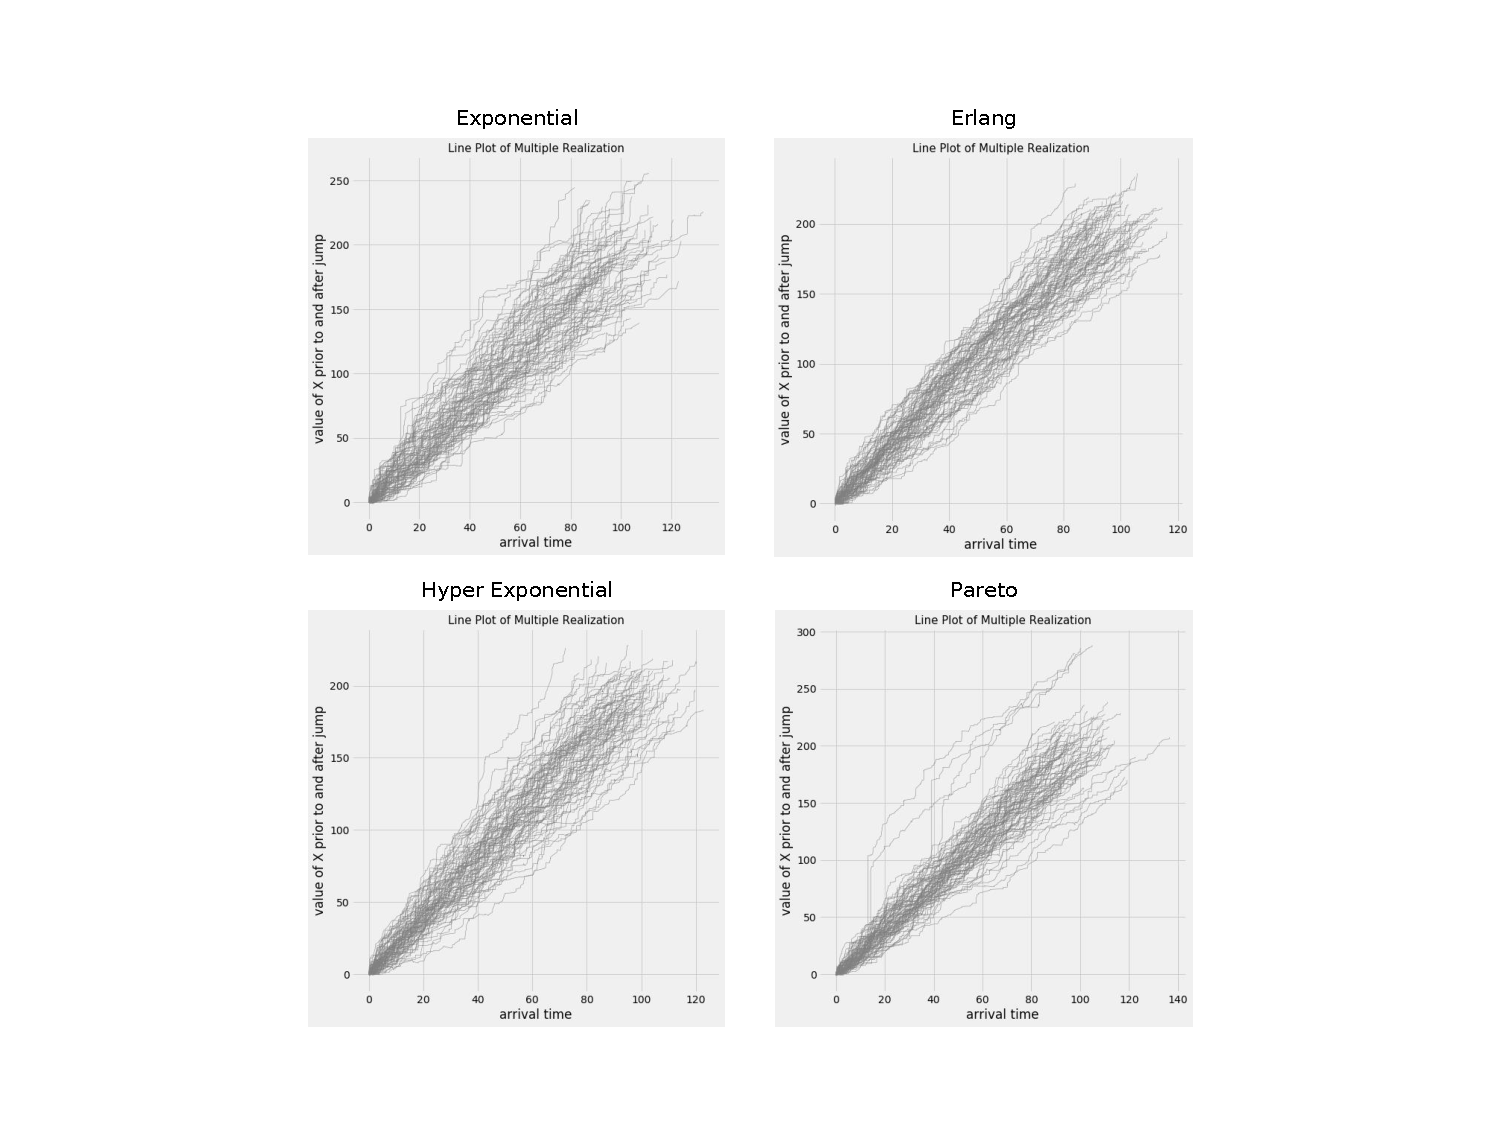
\includegraphics[scale = 0.9]{figures/task4.pdf}
    \caption{$Y_{i}$ following different $F$ distributions($\mu = 1$, $N_{jump} = 100$)}
    \label{fig:task4}
\end{figure}

\begin{itemize}
    \item Erlang distribution presents the lowest variance of path.
    \item Hyper-exponential distribution gives higher variance than the Exponential distribution.
    \item Pareto distribution often results in a higher probability of extreme observations, leading to large variance as well. Therefore, some paths on the bottom-right of figure \ref{fig:task4} have much longer jump at certain steps.
\end{itemize}

In order to examine the simulate value, the theoretical variance are calculated here:
\begin{enumerate}
    \item[(1)] Erlang distribution(k = 2):\\
    Combine two independent exponential variables with mean $\frac{1}{\lambda}$ each, then the variance is:\\
    $\mathbb{V}(X)=\frac{n}{\lambda^{2}} = \frac{2}{2^{2}} = \frac{1}{2}$
    
    \item[(2)] Exponential distribution:\\
    $\mathbb{V}(X)=\frac{1}{\lambda^{2}} = \frac{1}{1^2} = 1$ 
    
    \item[(3)] Hyper-exponential distribution:\\
    $\mathbb{V}(X) = \left[\sum_{i=1}^{n} \frac{p_{i}}{\lambda_{i}}\right]^{2}+\sum_{i=1}^{n} \sum_{j=1}^{n} p_{i} p_{j}\left(\frac{1}{\lambda_{i}}-\frac{1}{\lambda_{j}}\right)^{2}
    = 5.5$
    
    \item[(4)] Pareto distribution(k = 2):\\
    Because k is set to 2, then the variance of Pareto is infinite.
    
    
    
\end{enumerate}

Hence, the simulation accords with expected result of theory.









\newpage